%%Trying out a new ordering for the paper.
%%
%% This is file `sample-manuscript.tex',
%% generated with the docstrip utility.
%%
%% The original source files were:
%%
%% samples.dtx  (with options: `manuscript')
%% 
%% IMPORTANT NOTICE:
%% 
%% For the copyright see the source file.
%% 
%% Any modified versions of this file must be renamed
%% with new filenames distinct from sample-manuscript.tex.
%% 
%% For distribution of the original source see the terms
%% for copying and modification in the file samples.dtx.
%% 
%% This generated file may be distributed as long as the
%% original source files, as listed above, are part of the
%% same distribution. (The sources need not necessarily be
%% in the same archive or directory.)
%%
%% The first command in your LaTeX source must be the \documentclass command.
%%%% Small single column format, used for CIE, CSUR, DTRAP, JACM, JDIQ, JEA, JERIC, JETC, PACMCGIT, TAAS, TACCESS, TACO, TALG, TALLIP (formerly TALIP), TCPS, TDSCI, TEAC, TECS, TELO, THRI, TIIS, TIOT, TISSEC, TIST, TKDD, TMIS, TOCE, TOCHI, TOCL, TOCS, TOCT, TODAES, TODS, TOIS, TOIT, TOMACS, TOMM (formerly TOMCCAP), TOMPECS, TOMS, TOPC, TOPLAS, TOPS, TOS, TOSEM, TOSN, TQC, TRETS, TSAS, TSC, TSLP, TWEB.
% \documentclass[acmsmall]{acmart}

%%%% Large single column format, used for IMWUT, JOCCH, PACMPL, POMACS, TAP, PACMHCI
% \documentclass[acmlarge,screen]{acmart}

%%%% Large double column format, used for TOG
% \documentclass[acmtog, authorversion]{acmart}

%%%% Generic manuscript mode, required for submission
%%%% and peer review
\documentclass[manuscript,screen]{acmart}

%%
%% \BibTeX command to typeset BibTeX logo in the docs
\AtBeginDocument{%
  \providecommand\BibTeX{{%
    \normalfont B\kern-0.5em{\scshape i\kern-0.25em b}\kern-0.8em\TeX}}}

%% Rights management information.  This information is sent to you
%% when you complete the rights form.  These commands have SAMPLE
%% values in them; it is your responsibility as an author to replace
%% the commands and values with those provided to you when you
%% complete the rights form.
\setcopyright{acmcopyright}
\copyrightyear{2018}
\acmYear{2018}
\acmDOI{10.1145/1122445.1122456}

%% These commands are for a PROCEEDINGS abstract or paper.
%%\acmConference[Woodstock '18]{Woodstock '18: ACM Symposium on Neural
%%  Gaze Detection}{June 03--05, 2018}{Woodstock, NY}
%%\acmBooktitle{Woodstock '18: ACM Symposium on Neural Gaze Detection,
%%  June 03--05, 2018, Woodstock, NY}
%\acmPrice{15.00}
%\acmISBN{978-1-4503-XXXX-X/18/06}


%%
%% Submission ID.
%% Use this when submitting an article to a sponsored event. You'll
%% receive a unique submission ID from the organizers
%% of the event, and this ID should be used as the parameter to this command.
%%\acmSubmissionID{123-A56-BU3}

%%
%% The majority of ACM publications use numbered citations and
%% references.  The command \citestyle{authoryear} switches to the
%% "author year" style.
%%
%% If you are preparing content for an event
%% sponsored by ACM SIGGRAPH, you must use the "author year" style of
%% citations and references.
%% Uncommenting
%% the next command will enable that style.
%%\citestyle{acmauthoryear}

\usepackage{subcaption}
\usepackage{pgfplots}
\usepackage{pgfplotstable}

\DeclareMathOperator{\Div}{div}
\DeclareMathOperator{\curl}{curl}

\newcommand{\R}{\mathbb{R}}
\newcommand{\red}[1]{\textcolor{red}{#1}}
\newcommand{\akg}[1]{\textcolor{blue}{\textbf{AG:} #1}}

\newcommand{\calQ}{\mathcal{Q}}
\newcommand{\calS}{\mathcal{S}}

%%
%% end of the preamble, start of the body of the document source.
\begin{document}

%%
%% The "title" command has an optional parameter,
%% allowing the author to define a "short title" to be used in page headers.
\title{Bringing Trimmed Serendipity Methods to Computational Practice in Firedrake}

%%
%% The "author" command and its associated commands are used to define
%% the authors and their affiliations.
%% Of note is the shared affiliation of the first two authors, and the
%% "authornote" and "authornotemark" commands
%% used to denote shared contribution to the research.
\author{Cyrus Cheng}
\email{cyrus.cheng15@imperial.ac.uk}
\affiliation{%
  \institution{Imperial College}
  \city{London}
  \country{United Kingdom}
}

\author{Justin Crum}
\email{jcrum@math.arizona.edu}
\affiliation{%
  \institution{University of Arizona}
  \city{Tucson}
  \state{Arizona}
}

\author{Andrew Gillette}
\affiliation{%
  \institution{University of Arizona}
  \city{Tucson}
  \state{Arizona}}
\email{agillette@math.arizona.edu}

\author{David Ham}
\affiliation{%
  \institution{Imperial College}
  \city{London}
  \country{United Kingdom}
}
\email{david.ham@imperial.ac.uk}

\author{Robert Kirby}
\affiliation{%
 \institution{Baylor University}
 \city{Waco}
 \state{Texas}
}
\email{robert_kirby@baylor.edu}

\author{Joshua A. Levine}
\affiliation{%
  \institution{University of Arizona}
}
\email{josh@email.arizona.edu}

\author{Lawrence Mitchell}
\affiliation{%
  \institution{Durham University}
  \city{Durham}
  \country{United Kingdom}}
\email{wence@gmx.li}
%%
%% By default, the full list of authors will be used in the page
%% headers. Often, this list is too long, and will overlap
%% other information printed in the page headers. This command allows
%% the author to define a more concise list
%% of authors' names for this purpose.
%\renewcommand{\shortauthors}{Trovato and Tobin, et al.}

%%
%% The abstract is a short summary of the work to be presented in the
%% article.

\begin{abstract}
    An abstract about Firedrake and FEM here.
  \end{abstract}
  
  
  \maketitle
  
  
  \section{Introduction}
  
  \section{Background on serendipity and trimmed serendipity elements}
  
  \subsection{2D Elements}
  \begin{enumerate}
  \item Scalar (classical = Arnold-Awanou = $\calS_r\Lambda^0(\R^2)$)
  \item Vector Serendipity (BDM = Arnold-Awanou = $\calS_r\Lambda^1(\R^2)$)
  \item Vector Trimmed Serendipity (Arbogast-Correa = Gillette-Kloefkorn = $\calS_r^-\Lambda^1(\R^2)$)
  \item Direct (Arbogast-Tao / Arbogast-Correa)
  \end{enumerate}
  
  
  \subsubsection{Scalar (classical = Arnold-Awanou = $\calS_r\Lambda^0(\R^2)$)}
  
  \subsubsection{Vector Serendipity (BDM = Arnold-Awanou = $\calS_r\Lambda^1(\R^2)$)}
  
  \subsubsection{Vector Trimmed Serendipity (Arbogast-Correa = Gillette-Kloefkorn = $\calS_r^-\Lambda^1(\R^2)$)}
  
  \subsubsection{Direct (Arbogast-Tao / Arbogast-Correa)}
  
  \subsection{3D Elements}
  \begin{enumerate}
  \item Scalar (classical = Arnold-Awanou = $\calS_r\Lambda^0(\R^3)$)
  \item Vector serendipity (Arnold-Awanou = $\calS_r\Lambda^1(\R^3)$ and $\calS_r\Lambda^2(\R^3)$
  \item Vector trimmed serendipity (Gillette-Kloefkorn = $\calS_r^-\Lambda^1(\R^3)$ and $\calS_r^-\Lambda^2(\R^3)$)
  
  \end{enumerate}
  
  \section{Building capacity for serendipity element types in Firedrake}
  
  Firedrake is a python package that is made to solve finite element problems.  It does this by tying together many packages in a cohesive manner.  For implementing a new finite element, we can focus on a few specific packages, namely FIAT, FInAT, UFL, and TSFC.  
  
  \noindent First, we use the UFL package.  This is a symbolic math package that implemented the Unified Form Language in Python.  Specifically, UFL allows Firedrake to specify a PDE in weak form that we then want to solve.  Next, FIAT (FInite element Automatic Tabulator) allows a simple Ciarlet implementation of finite elements that makes the process of adding in new types of elements a relatively simple task.  On the other hand, FInAT (FInAT Is not A Tabulator) is a way to pass symbolic for evaluation of finite elements.  What FInAT gives out can then be handled by a form compiler.  The form compiler that Firedrake uses is TSFC (Two Stage Form Compiler), and is used to take the high level, weak form PDE and turn it into low level code that can be solved.  
  
  \noindent Implementing a new element, like the trimmed Serendipity elements in 2 and 3D, then becomes a matter of adding in a new element code to FIAT, telling UFL what to expect when we call the new element (i.e., what type of shapes does it work on, what dimensions does it work in, what type of element it is), and connecting the dots in FInAT and TSFC.  Starting off in the FIAT portion of the code, we create a new element by making a call to the FiniteElement class.  In this class, we give the relevant information for describing a reference element of the type we're choosing.  For example, we need to give it the number of degrees of freedom on each edge and face, and then we need to build and assign basis functions to each of the degrees of freedom.   Once done, the rest of the code is designed for passing around the new element from library to library.  We import the fiat element to FInAT so that it knows of the existence of the new element.  Then we tell TSFC where to find the new element, and give it a name that a Firedrake user can give when calling the element.  Finally, we give UFL the directions of what sort of elements we are allowed to use the new finite element on.    
  

  \section{Experiments}
    
   The following experiments were designed to show the benefits and costs to using trimmed Serendipity elements in comparison to traditional tensor product elements.  We used a basic projection example to check implementation, as well as a primal Poisson problem (to test scalar elements), a mixed Poisson problem (to test H(div) elements), and a cavity resonator problem (to test H(curl) elements).  Note that the cavity resonator problem was done only in 3D, as in 2D, the H(curl) elements are just a rotation of the H(div) elements. 

\newpage
  \subsection{Projection}
  
  We solve the projection problem to give a baseline of expectations for the elements.  
  
  GET THE EXACT PROBLEM THAT THE PROJECTION PROBLEM IS SOLVING.

\begin{figure}[h!]
  \begin{subfigure}[h]{0.5\textwidth}
    %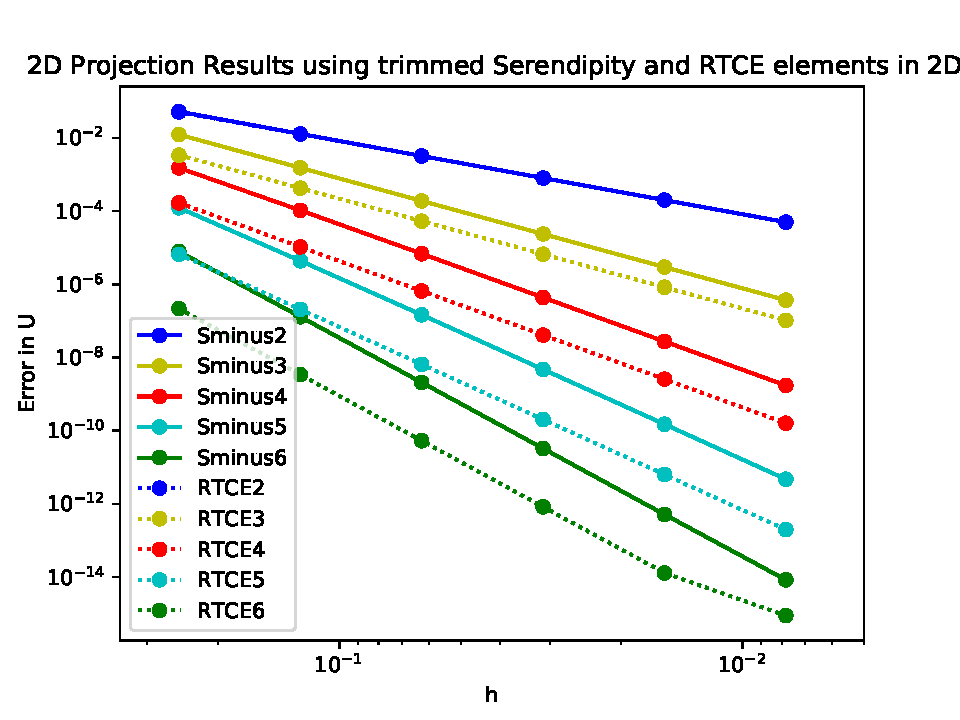
\includegraphics[height=2.2in]{2dProjectionH.pdf}
    \begin{tikzpicture}[scale=0.88]
      \begin{loglogaxis}[xlabel={h}, ylabel={Error},
             ylabel near ticks, ymax=1e-1, ymin=2e-11, xmax=0.3, xmin=0.5e-2,
             legend pos=south east, legend style={font=\tiny} ,
             cycle list name=color list, title={Projection Error Analysis in 2D}]
        %\addplot+[only marks, orange] table [x=Dofs,y=Time,col sep=comma]{PrimalPoissonSerendipity3dO4.csv};
        \addplot[red]
        table [x=h,y=Error, col sep=comma]{ProjectionSminus2dO2.csv};
        \addlegendentry{$S^-_2$}
        \addplot[blue] 
        table [x=h,y=Error, col sep=comma]{ProjectionSminus2dO3.csv};
        \addlegendentry{$S^-_3$ }
        \addplot[orange]
        table [x=h,y=Error, col sep=comma]{ProjectionSminus2dO4.csv};
        \addlegendentry{$S^-_4$}
        \addplot[densely dotted, red]
        table [x=h,y=Error, col sep=comma]{ProjectionRTCE2dO2.csv};
        \addlegendentry{$Q^-_2$}
        \addplot[densely dotted, blue] 
        table [x=h,y=Error, col sep=comma]{ProjectionRTCE2dO3.csv};
        \addlegendentry{$Q^-_3$}
        \addplot[densely dotted, orange]
        table [x=h,y=Error, col sep=comma]{ProjectionRTCE2dO4.csv};
        \addlegendentry{$Q^-_4$}
        
        \addplot+[only marks, red] table [x=h,y=Error,col sep=comma]{ProjectionSminus2dO2.csv};
        \addplot+[only marks, red, mark=square*] table [x=h,y=Error,col sep=comma]{ProjectionRTCE2dO2.csv};
        \addplot+[only marks, blue] table [x=h,y=Error,col sep=comma]{ProjectionSminus2dO3.csv};
        \addplot+[only marks, blue, mark=square*] table [x=h,y=Error,col sep=comma]{ProjectionRTCE2dO3.csv};
        \addplot+[only marks, orange] table [x=h,y=Error,col sep=comma]{ProjectionSminus2dO4.csv};
        \addplot+[only marks, orange, mark=square*] table [x=h,y=Error,col sep=comma]{ProjectionRTCE2dO4.csv};
      \end{loglogaxis}
      \end{tikzpicture}
    \caption{2D edge length vs error}
    \label{fig:2dProjectionH}
  \end{subfigure}
  ~
  \begin{subfigure}[h]{0.5\textwidth}
     %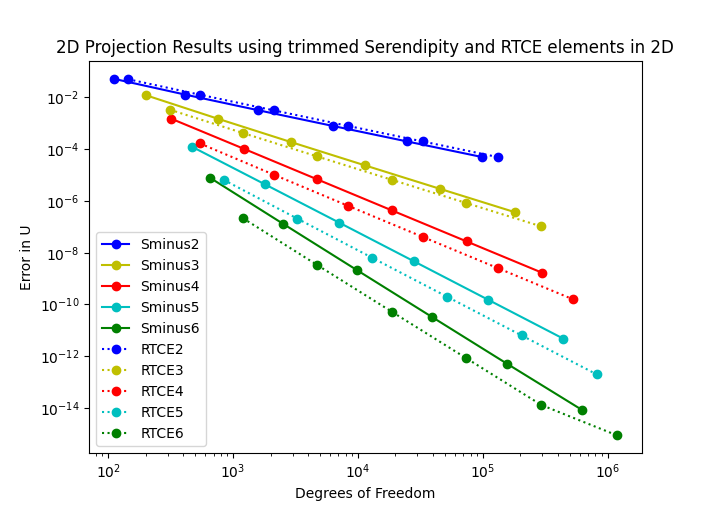
\includegraphics[height=2.2in]{2dProjection.png}
     \begin{tikzpicture}[scale=0.88]
      \begin{loglogaxis}[xlabel={Degrees of Freedom}, ylabel={Error},
             ylabel near ticks, ymax=1e-1, ymin=2e-11, xmax=3e6, xmin=0.5e2,
             legend pos=south west, legend style={font=\tiny} ,
             cycle list name=color list, title={Projection Error Analysis in 2D}]
        %\addplot+[only marks, orange] table [x=Dofs,y=Time,col sep=comma]{PrimalPoissonSerendipity3dO4.csv};
        \addplot[red]
        table [x=Dofs,y=Error, col sep=comma]{ProjectionSminus2dO2.csv};
        \addlegendentry{$S^-_2$}
        \addplot[blue] 
        table [x=Dofs,y=Error, col sep=comma]{ProjectionSminus2dO3.csv};
        \addlegendentry{$S^-_3$ }
        \addplot[orange]
        table [x=Dofs,y=Error, col sep=comma]{ProjectionSminus2dO4.csv};
        \addlegendentry{$S^-_4$}
        \addplot[densely dotted, red]
        table [x=Dofs,y=Error, col sep=comma]{ProjectionRTCE2dO2.csv};
        \addlegendentry{$Q^-_2$}
        \addplot[densely dotted, blue] 
        table [x=Dofs,y=Error, col sep=comma]{ProjectionRTCE2dO3.csv};
        \addlegendentry{$Q^-_3$}
        \addplot[densely dotted, orange]
        table [x=Dofs,y=Error, col sep=comma]{ProjectionRTCE2dO4.csv};
        \addlegendentry{$Q^-_4$}
        
        \addplot+[only marks, red] table [x=Dofs,y=Error,col sep=comma]{ProjectionSminus2dO2.csv};
        \addplot+[only marks, red, mark=square*] table [x=Dofs,y=Error,col sep=comma]{ProjectionRTCE2dO2.csv};
        \addplot+[only marks, blue] table [x=Dofs,y=Error,col sep=comma]{ProjectionSminus2dO3.csv};
        \addplot+[only marks, blue, mark=square*] table [x=Dofs,y=Error,col sep=comma]{ProjectionRTCE2dO3.csv};
        \addplot+[only marks, orange] table [x=Dofs,y=Error,col sep=comma]{ProjectionSminus2dO4.csv};
        \addplot+[only marks, orange, mark=square*] table [x=Dofs,y=Error,col sep=comma]{ProjectionRTCE2dO4.csv};
      \end{loglogaxis}
      \end{tikzpicture}
     \caption{2D degrees of freedom vs error}
     \label{fig:2dProjection}
  \end{subfigure} \\
  ~
  \begin{subfigure}[h]{0.5\textwidth}
    \begin{tikzpicture}[scale=0.88]
      \begin{loglogaxis}[xlabel={h}, ylabel={Error},
             ylabel near ticks, ymax=1e-1, ymin=2e-10, xmax=0.2, xmin=0.5e-2,
             legend pos=south east, legend style={font=\tiny} ,
             cycle list name=color list, title={Projection Error Analysis in 3D}]
        %\addplot+[only marks, orange] table [x=Dofs,y=Time,col sep=comma]{PrimalPoissonSerendipity3dO4.csv};
        \addplot[red]
        table [x=h,y=Error, col sep=comma]{ProjectionSminus3dO2.csv};
        \addlegendentry{$S^-_2$}
        \addplot[blue] 
        table [x=h,y=Error, col sep=comma]{ProjectionSminus3dO3.csv};
        \addlegendentry{$S^-_3$ }
        \addplot[orange]
        table [x=h,y=Error, col sep=comma]{ProjectionSminus3dO4.csv};
        \addlegendentry{$S^-_4$}
        \addplot[densely dotted, red]
        table [x=h,y=Error, col sep=comma]{ProjectionNCE3dO2.csv};
        \addlegendentry{$Q^-_2$}
        \addplot[densely dotted, blue] 
        table [x=h,y=Error, col sep=comma]{ProjectionNCE3dO3.csv};
        \addlegendentry{$Q^-_3$}
        \addplot[densely dotted, orange]
        table [x=h,y=Error, col sep=comma]{ProjectionNCE3dO4.csv};
        \addlegendentry{$Q^-_4$}
        
        \addplot+[only marks, red] table [x=h,y=Error,col sep=comma]{ProjectionSminus3dO2.csv};
        \addplot+[only marks, red, mark=square*] table [x=h,y=Error,col sep=comma]{ProjectionNCE3dO2.csv};
        \addplot+[only marks, blue] table [x=h,y=Error,col sep=comma]{ProjectionSminus3dO3.csv};
        \addplot+[only marks, blue, mark=square*] table [x=h,y=Error,col sep=comma]{ProjectionNCE3dO3.csv};
        \addplot+[only marks, orange] table [x=h,y=Error,col sep=comma]{ProjectionSminus3dO4.csv};
        \addplot+[only marks, orange, mark=square*] table [x=h,y=Error,col sep=comma]{ProjectionNCE3dO4.csv};
      \end{loglogaxis}
      \end{tikzpicture}
    %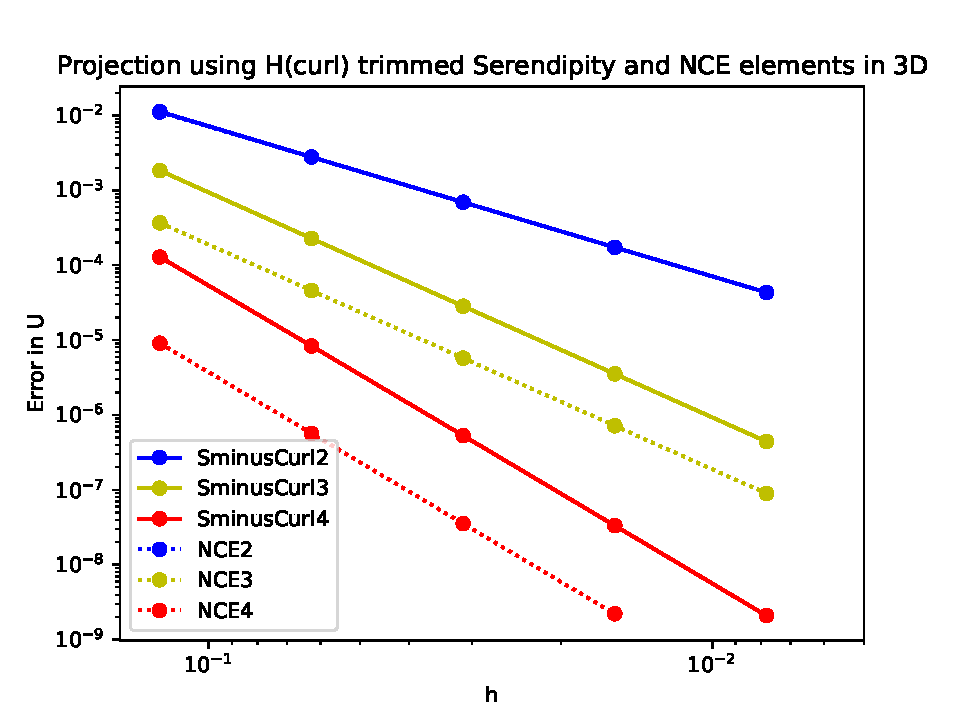
\includegraphics[height=2.2in]{3dProjectionHError.pdf}
    \caption{3D edge length vs error}
    \label{fig:3dProjectionH}
  \end{subfigure}
  ~
  \begin{subfigure}[h]{0.5\textwidth}
  \begin{tikzpicture}[scale=0.88]
      \begin{loglogaxis}[xlabel={Degrees of Freedom}, ylabel={Error},
             ylabel near ticks, ymax=3e-2, ymin=0.5e-9, xmax=4e8, xmin=0.25e4,
             legend pos=south west, legend style={font=\tiny} ,
             cycle list name=color list, title={Projection Error Analysis in 3D}]
        %\addplot+[only marks, orange] table [x=Dofs,y=Time,col sep=comma]{PrimalPoissonSerendipity3dO4.csv};
        \addplot[red]
        table [x=Dofs,y=Error, col sep=comma]{ProjectionSminus3dO2.csv};
        \addlegendentry{$S^-_2$}
        \addplot[blue] 
        table [x=Dofs,y=Error, col sep=comma]{ProjectionSminus3dO3.csv};
        \addlegendentry{$S^-_3$ }
        \addplot[orange]
        table [x=Dofs,y=Error, col sep=comma]{ProjectionSminus3dO4.csv};
        \addlegendentry{$S^-_4$}
        \addplot[densely dotted, red]
        table [x=Dofs,y=Error, col sep=comma]{ProjectionNCE3dO2.csv};
        \addlegendentry{$Q^-_2$}
        \addplot[densely dotted, blue] 
        table [x=Dofs,y=Error, col sep=comma]{ProjectionNCE3dO3.csv};
        \addlegendentry{$Q^-_3$}
        \addplot[densely dotted, orange]
        table [x=Dofs,y=Error, col sep=comma]{ProjectionNCE3dO4.csv};
        \addlegendentry{$Q^-_4$}
        
        \addplot+[only marks, red] table [x=Dofs,y=Error,col sep=comma]{ProjectionSminus3dO2.csv};
        \addplot+[only marks, red, mark=square*] table [x=Dofs,y=Error,col sep=comma]{ProjectionNCE3dO2.csv};
        \addplot+[only marks, blue] table [x=Dofs,y=Error,col sep=comma]{ProjectionSminus3dO3.csv};
        \addplot+[only marks, blue, mark=square*] table [x=Dofs,y=Error,col sep=comma]{ProjectionNCE3dO3.csv};
        \addplot+[only marks, orange] table [x=Dofs,y=Error,col sep=comma]{ProjectionSminus3dO4.csv};
        \addplot+[only marks, orange, mark=square*] table [x=Dofs,y=Error,col sep=comma]{ProjectionNCE3dO4.csv};
      \end{loglogaxis}
      \end{tikzpicture}
    %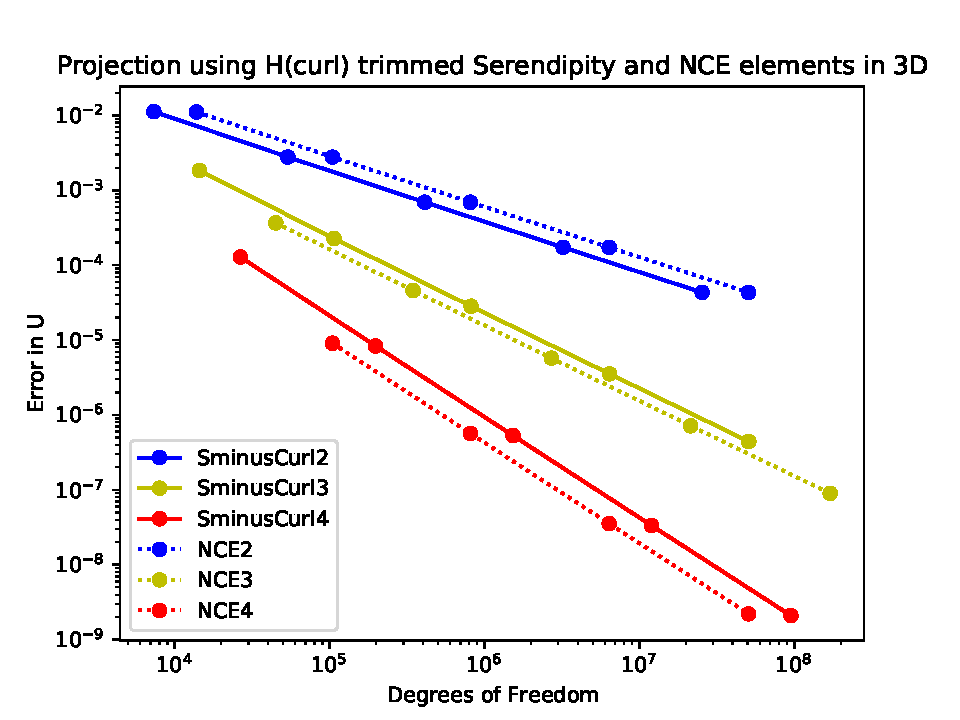
\includegraphics[height=2.2in]{3dProjectionDofsError.pdf}
    \caption{3D degrees of freedom vs error}
    \label{fig:3dProjectionDofs}
  \end{subfigure}
  \caption{Results of solving projection problem using 2D and 3D $S^-$ curl elements and tensor product curl elements.}
\end{figure}
  
First, we graphed the errors from computing projections using trimmed Serendipity and tensor product elements in 2D, shown in Figure \ref{fig:2dProjectionH}.  Since we expect that the order of convergence for both of these elements should be the same (only off by a constant factor), we look for the lines representing trimmed Serendipity and tensor product elements at a given order to be parallel.
  
After checking that it is converging at the right rate, we then want to analyze the data from a standpoint of memory usage.  To do this, we plot degrees of freedom vs error, as seen in Figure \ref{fig:2dProjection}.  Overall, the error given by trimmed Serendipity elements is higher than the error from using tensor product elements of the same order.   We see similar results in Figures \ref{fig:3dProjectionDofs} and \ref{fig:3dProjectionH}.
  


\newpage
 
\subsection{The Poisson Problem}
In this section we discuss results for both the primal Poisson problem as well as the mixed Poisson problem.  We solve the primal Poisson problem described below on a unit square domain $\Omega$:
\begin{align}
    -\nabla^2 u &= f \\
    u\vert_{\partial \Omega} &= 0 \\
    \nabla u \cdot n &= 0 \text{ on } \partial \Omega
\end{align}
where $f(x,y) = 2\pi^2\text{sin}(\pi x)\text{sin}(\pi y) $, yielding the solution $u(x,y) = \text{sin}(\pi x)\text{sin}(\pi y)$. In 3D, we can extend this to $f(x,y,z) = 2\pi^2\text{sin}(\pi x)\text{sin}(\pi y)\text{sin}(\pi z)$ with the solution being $u(x,y,z) = \text{sin}(\pi x)\text{sin}(\pi y)\text{sin}(\pi z)$.  

The primal Poisson problem allows us to test scalar Serendipity elements against Lagrange elements.  Then we wish to also test H(div) elements.  To do this, we solve a discretization of the mixed Poisson problem:

\begin{align}
     \sigma - \nabla u &= 0 \\
     \nabla \cdot \sigma &= -f \notag \\
     u\vert_{\partial \Omega} &= 0 \notag
\end{align}


\begin{figure}[h!]
  \centering
  \begin{subfigure}[h]{0.5\textwidth}
    \centering
      \begin{tikzpicture}[scale=0.88]
      \begin{loglogaxis}[xlabel={Degrees of Freedom}, ylabel={Error},
             ylabel near ticks, ymax=1e-4, ymin=1e-16, xmax=2e6, xmin=2e3,
             legend pos=south west, legend style={font=\tiny} ,
             cycle list name=color list, title={Primal Poisson Error Analysis}]
        %\addplot+[only marks, orange] table [x=Dofs,y=Time,col sep=comma]{PrimalPoissonSerendipity3dO4.csv};
        \addplot[red]
        table [x=Dofs,y=Error, col sep=comma]{PrimalPoissonSerendipity2dO2.csv};
        \addlegendentry{$S^-_2$}
        \addplot[blue] 
        table [x=Dofs,y=Error, col sep=comma]{PrimalPoissonSerendipity2dO3.csv};
        \addlegendentry{$S^-_3$ }
        \addplot[orange]
        table [x=Dofs,y=Error, col sep=comma]{PrimalPoissonSerendipity2dO4.csv};
        \addlegendentry{$S^-_4$}
        \addplot[densely dotted, red]
        table [x=Dofs,y=Error, col sep=comma]{PrimalPoissonLagrange2dO2.csv};
        \addlegendentry{$Q^-_2$}
        \addplot[densely dotted, blue] 
        table [x=Dofs,y=Error, col sep=comma]{PrimalPoissonLagrange2dO3.csv};
        \addlegendentry{$Q^-_3$}
        \addplot[densely dotted, orange]
        table [x=Dofs,y=Error, col sep=comma]{PrimalPoissonLagrange2dO4.csv};
        \addlegendentry{$Q^-_4$}
        
        \addplot+[only marks, red] table [x=Dofs,y=Error,col sep=comma]{PrimalPoissonSerendipity2dO2.csv};
        \addplot+[only marks, red, mark=square*] table [x=Dofs,y=Error,col sep=comma]{PrimalPoissonLagrange2dO2.csv};
        \addplot+[only marks, blue] table [x=Dofs,y=Error,col sep=comma]{PrimalPoissonSerendipity2dO3.csv};
        \addplot+[only marks, blue, mark=square*] table [x=Dofs,y=Error,col sep=comma]{PrimalPoissonLagrange2dO3.csv};
        \addplot+[only marks, orange] table [x=Dofs,y=Error,col sep=comma]{PrimalPoissonSerendipity2dO4.csv};
        \addplot+[only marks, orange, mark=square*] table [x=Dofs,y=Error,col sep=comma]{PrimalPoissonLagrange2dO4.csv};
      \end{loglogaxis}
      \end{tikzpicture}
    %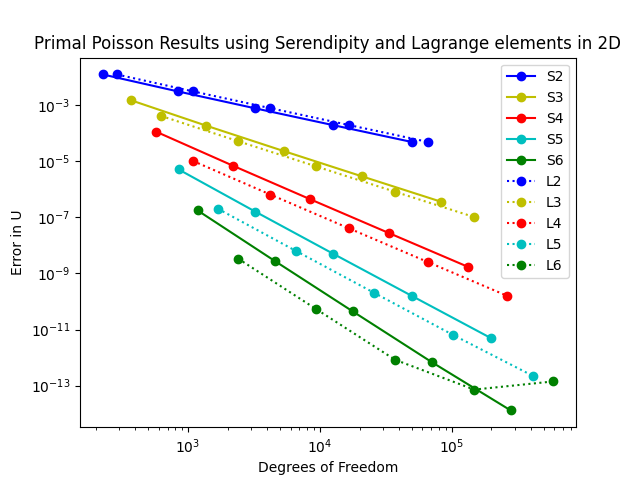
\includegraphics[height=2.2in]{2dPrimalPoisson.png}
    \caption{2D Primal}
    \label{fig:2dPrimalDofs}
  \end{subfigure}
  ~
  \begin{subfigure}[h]{0.5\textwidth}
    \centering
    \begin{tikzpicture}[scale=0.88]
      \begin{loglogaxis}[xlabel={Degrees of Freedom}, ylabel={Error},
             ylabel near ticks, ymax=1e-1, ymin=1e-11, xmax=2e6, xmin=3e2,
             legend pos=south west, legend style={font=\tiny} ,
             cycle list name=color list, title={Mixed Poisson Error Analysis}]
        %\addplot+[only marks, orange] table [x=Dofs,y=Time,col sep=comma]{PrimalPoissonSerendipity3dO4.csv};
        \addplot[red]
        table [x=Dofs,y=Error, col sep=comma]{MixedPoissonSminus2dO2.csv};
        \addlegendentry{$S^-_2$}
        \addplot[blue] 
        table [x=Dofs,y=Error, col sep=comma]{MixedPoissonSminus2dO3.csv};
        \addlegendentry{$S^-_3$ }
        \addplot[orange]
        table [x=Dofs,y=Error, col sep=comma]{MixedPoissonSminus2dO4.csv};
        \addlegendentry{$S^-_4$}
        \addplot[densely dotted, red]
        table [x=Dofs,y=Error, col sep=comma]{MixedPoissonRTCF2dO2.csv};
        \addlegendentry{$Q^-_2$}
        \addplot[densely dotted, blue] 
        table [x=Dofs,y=Error, col sep=comma]{MixedPoissonRTCF2dO3.csv};
        \addlegendentry{$Q^-_3$}
        \addplot[densely dotted, orange]
        table [x=Dofs,y=Error, col sep=comma]{MixedPoissonRTCF2dO4.csv};
        \addlegendentry{$Q^-_4$}
        
        \addplot+[only marks, red] table [x=Dofs,y=Error,col sep=comma]{MixedPoissonSminus2dO2.csv};
        \addplot+[only marks, red, mark=square*] table [x=Dofs,y=Error,col sep=comma]{MixedPoissonRTCF2dO2.csv};
        \addplot+[only marks, blue] table [x=Dofs,y=Error,col sep=comma]{MixedPoissonSminus2dO3.csv};
        \addplot+[only marks, blue, mark=square*] table [x=Dofs,y=Error,col sep=comma]{MixedPoissonRTCF2dO3.csv};
        \addplot+[only marks, orange] table [x=Dofs,y=Error,col sep=comma]{MixedPoissonSminus2dO4.csv};
        \addplot+[only marks, orange, mark=square*] table [x=Dofs,y=Error,col sep=comma]{MixedPoissonRTCF2dO4.csv};
      \end{loglogaxis}
      \end{tikzpicture}
    %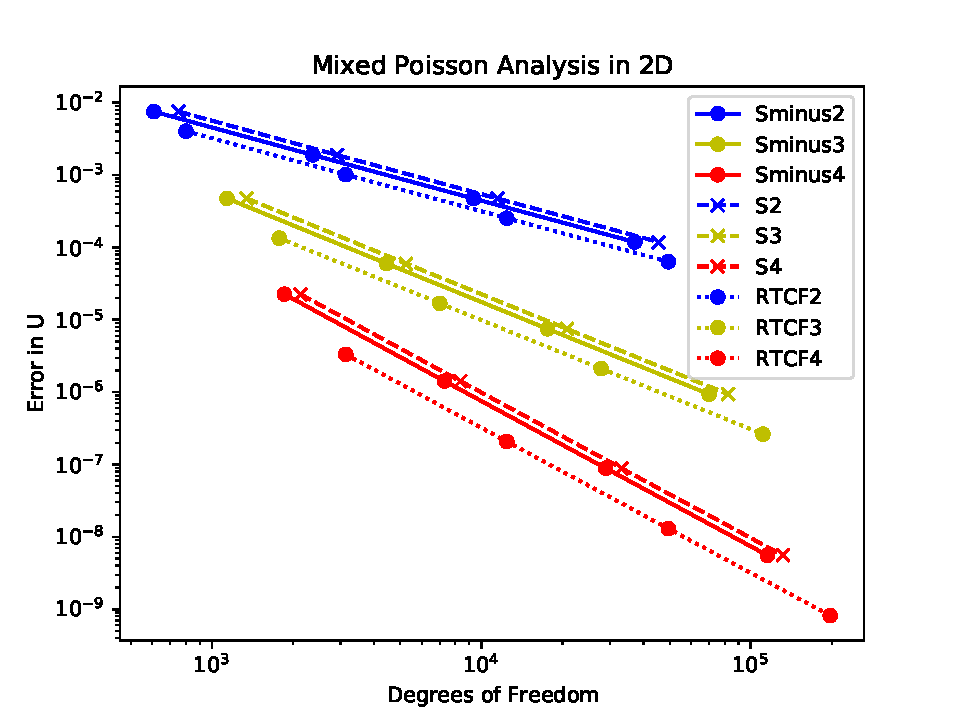
\includegraphics[height=2.2in]{2dMixedPoissonDofs.pdf}
    \caption{2D Mixed}
    \label{fig:2dMixedDofsError}
  \end{subfigure} \\
  \begin{subfigure}[h]{0.5\textwidth}
    \centering
    \begin{tikzpicture}[scale=0.88]
      \begin{loglogaxis}[xlabel={Degrees of Freedom}, ylabel={Error},
             ylabel near ticks, ymax=1e-3, ymin=1e-11, xmax=2e8, xmin=1e3,
             legend pos=south west, legend style={font=\tiny} ,
             cycle list name=color list, title={Primal Poisson Error Analysis}]
        %\addplot+[only marks, orange] table [x=Dofs,y=Time,col sep=comma]{PrimalPoissonSerendipity3dO4.csv};
        \addplot[red]
        table [x=Dofs,y=Error, col sep=comma]{PrimalPoissonSerendipity3dO2.csv};
        \addlegendentry{$S^-_2$}
        \addplot[blue] 
        table [x=Dofs,y=Error, col sep=comma]{PrimalPoissonSerendipity3dO3.csv};
        \addlegendentry{$S^-_3$ }
        \addplot[orange]
        table [x=Dofs,y=Error, col sep=comma]{PrimalPoissonSerendipity3dO4.csv};
        \addlegendentry{$S^-_4$}
        \addplot[densely dotted, red]
        table [x=Dofs,y=Error, col sep=comma]{PrimalPoissonLagrange3dO2.csv};
        \addlegendentry{$Q^-_2$}
        \addplot[densely dotted, blue] 
        table [x=Dofs,y=Error, col sep=comma]{PrimalPoissonLagrange3dO3.csv};
        \addlegendentry{$Q^-_3$}
        \addplot[densely dotted, orange]
        table [x=Dofs,y=Error, col sep=comma]{PrimalPoissonLagrange3dO4.csv};
        \addlegendentry{$Q^-_4$}
        
        \addplot+[only marks, red] table [x=Dofs,y=Error,col sep=comma]{PrimalPoissonSerendipity3dO2.csv};
        \addplot+[only marks, red, mark=square*] table [x=Dofs,y=Error,col sep=comma]{PrimalPoissonLagrange3dO2.csv};
        \addplot+[only marks, blue] table [x=Dofs,y=Error,col sep=comma]{PrimalPoissonSerendipity3dO3.csv};
        \addplot+[only marks, blue, mark=square*] table [x=Dofs,y=Error,col sep=comma]{PrimalPoissonLagrange3dO3.csv};
        \addplot+[only marks, orange] table [x=Dofs,y=Error,col sep=comma]{PrimalPoissonSerendipity3dO4.csv};
        \addplot+[only marks, orange, mark=square*] table [x=Dofs,y=Error,col sep=comma]{PrimalPoissonLagrange3dO4.csv};
      \end{loglogaxis}
      \end{tikzpicture}
    %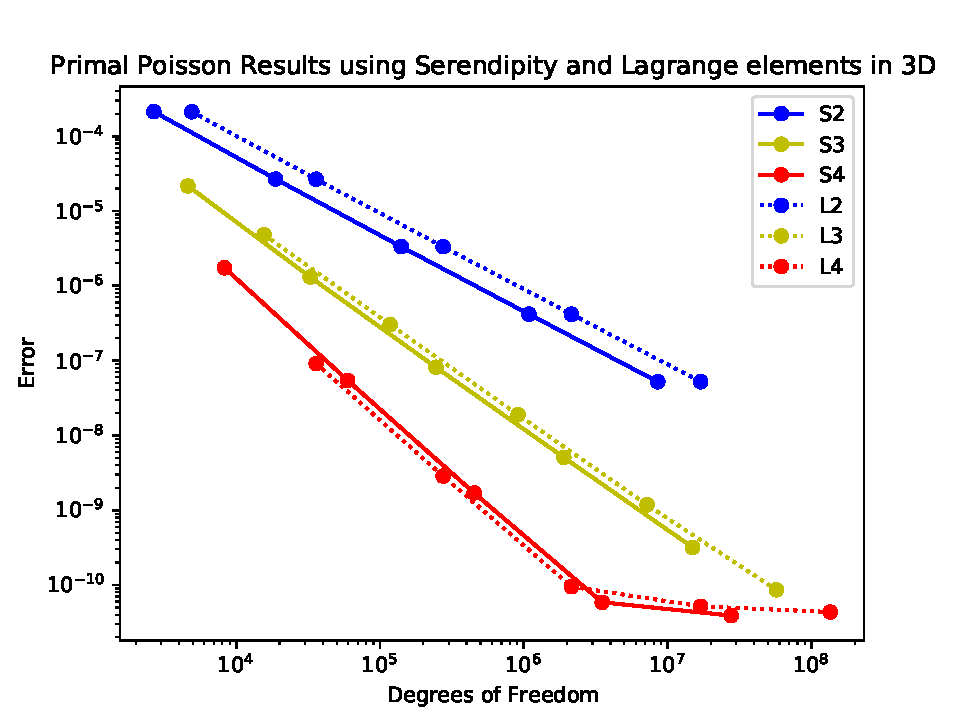
\includegraphics[height=2.2in]{3dPrimalDofsError.pdf}
    \caption{3D Primal}
    \label{fig:3dPrimalDofsError}
  \end{subfigure}
  ~
  \begin{subfigure}[h]{0.5\textwidth}
    \centering
    %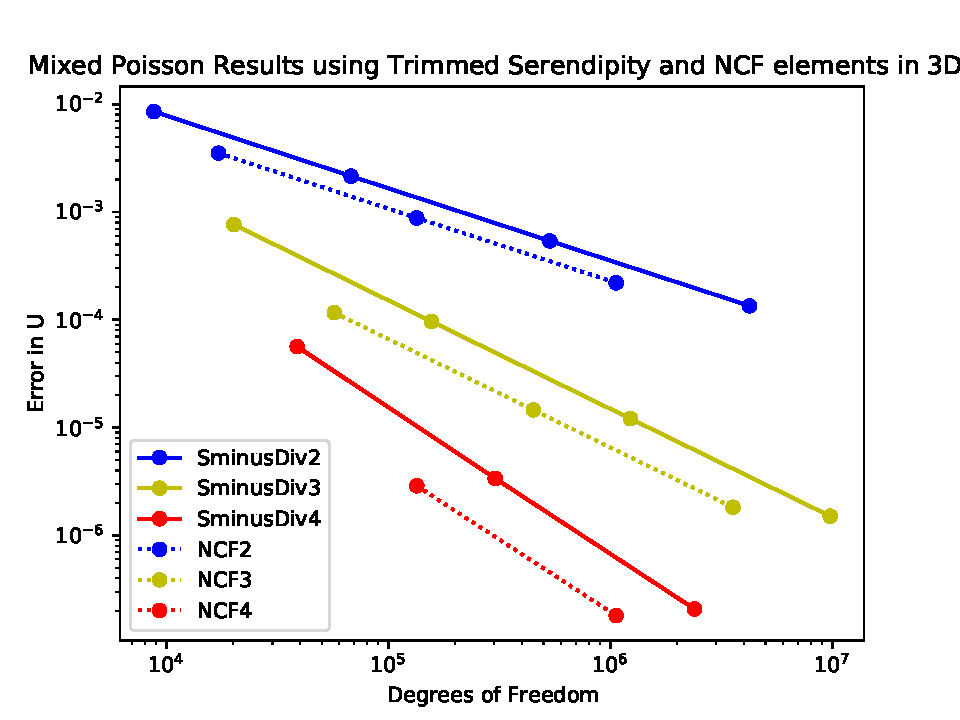
\includegraphics[height=2.2in]{3dMixedPoissonDofsError.pdf}
    \begin{tikzpicture}[scale=0.88]
      \begin{loglogaxis}[xlabel={Degrees of Freedom}, ylabel={Error},
             ylabel near ticks, ymax=1.2e-2, ymin=0.8e-7, xmax=2e7, xmin=5e3,
             legend pos=south west, legend style={font=\tiny} ,
             cycle list name=color list, title={Mixed Poisson Error Analysis}]
        %\addplot+[only marks, orange] table [x=Dofs,y=Time,col sep=comma]{PrimalPoissonSerendipity3dO4.csv};
        \addplot[red]
        table [x=Dofs,y=Error, col sep=comma]{MixedPoissonSminus3dO2.csv};
        \addlegendentry{$S^-_2$}
        \addplot[blue] 
        table [x=Dofs,y=Error, col sep=comma]{MixedPoissonSminus3dO3.csv};
        \addlegendentry{$S^-_3$ }
        \addplot[orange]
        table [x=Dofs,y=Error, col sep=comma]{MixedPoissonSminus3dO4.csv};
        \addlegendentry{$S^-_4$}
        \addplot[densely dotted, red]
        table [x=Dofs,y=Error, col sep=comma]{MixedPoissonNCF3dO2.csv};
        \addlegendentry{$Q^-_2$}
        \addplot[densely dotted, blue] 
        table [x=Dofs,y=Error, col sep=comma]{MixedPoissonNCF3dO3.csv};
        \addlegendentry{$Q^-_3$}
        \addplot[densely dotted, orange]
        table [x=Dofs,y=Error, col sep=comma]{MixedPoissonNCF3dO4.csv};
        \addlegendentry{$Q^-_4$}
        
        \addplot+[only marks, red] table [x=Dofs,y=Error,col sep=comma]{MixedPoissonSminus3dO2.csv};
        \addplot+[only marks, red, mark=square*] table [x=Dofs,y=Error,col sep=comma]{MixedPoissonNCF3dO2.csv};
        \addplot+[only marks, blue] table [x=Dofs,y=Error,col sep=comma]{MixedPoissonSminus3dO3.csv};
        \addplot+[only marks, blue, mark=square*] table [x=Dofs,y=Error,col sep=comma]{MixedPoissonNCF3dO3.csv};
        \addplot+[only marks, orange] table [x=Dofs,y=Error,col sep=comma]{MixedPoissonSminus3dO4.csv};
        \addplot+[only marks, orange, mark=square*] table [x=Dofs,y=Error,col sep=comma]{MixedPoissonNCF3dO4.csv};
      \end{loglogaxis}
      \end{tikzpicture}
    \caption{3D Mixed}
    \label{fig:3dMixedDofsError}
  \end{subfigure}
  \caption{An error analysis of the primal and mixed Poisson problems in 2D and 3D.}
\label{fig:PrimalMixedErrorAnalysis}
\end{figure}


Figures \ref{fig:2dPrimalDofs}, \ref{fig:2dMixedDofsError}, \ref{fig:3dPrimalDofsError}, and \ref{fig:3dMixedDofsError} give us some interesting data points to focus on.  Before analyzing the results, note again that Serendipity and trimmed Serendipity elements are the same in the primal Poisson case.  While these elements differ in the H(div) and H(curl) cases, our results here indicate that we likely will not see Serendiptiy elements outperforming trimmed Serendipity elements in 3D, so their implementation has been left for a future work.

In each of the figures in \ref{fig:PrimalMixedErrorAnalysis}, we see that regardless of which element is better, they follow similar trajectories again, indicating that they have the same overall convergence rate.  The primal Poisson problem shows us that there are scenarios where using Serendipity elements can be beneficial in terms of error depending on the number of degrees of freedom.  However, in the mixed Poisson problem, we don't immediately see this benefit in either the 2D case or the 3D case.

However, we would also like to analyze timing for tensor product elements and trimmed Serendipity elements.  We do this in the subfigures of \ref{fig:PrimalMixedTimeAnalysis}.  In \ref{fig:3dPrimalDofsTime} and \ref{fig:3dPrimalTimeError}, we see good evidence that Serendipity elements are able to to produce better results at a faster rate.  Specifically, in \ref{fig:3dPrimalDofsTime}, we can see that Serendipity elements are able to do a larger number of degrees of freedom in the same amount of time.  In fig \ref{fig:3dPrimalTimeError} we see that for a given error level, Serendipity elements require less time.

However the picture that is painted in \ref{fig:3dMixedDofsTime} and \ref{fig:3dMixedTimeError} is much less clear.  Overall, trimmed Serendipity elements seem to do a bit worse than the corresponding tensor product elements for the mixed Poisson problem, but it is promising that in \ref{fig:3dMixedDofsTime}, the points tend to stay in an overall linear fashion bunched together. 

\newpage

\begin{figure}[ht]
  \centering
  \begin{subfigure}[h]{0.5\textwidth}
    \centering
          \begin{tikzpicture}[scale=0.88]
      \begin{loglogaxis}[xlabel={Degrees of Freedom}, ylabel={Time},
             ylabel near ticks, ymax=1.e+4, ymin=0.5e-1, xmax=2.e8, xmin=1.e+3,
             legend pos=north west, legend style={font=\tiny} ,
             cycle list name=color list, title={Primal Poisson using $S^-$ and $Q^-$}]
        %\addplot+[only marks, orange] table [x=Dofs,y=Time,col sep=comma]{PrimalPoissonSerendipity3dO4.csv};
        \addplot[red]
        table [x=Dofs,y=Time, col sep=comma]{PrimalPoissonSerendipity3dO2.csv};
        \addlegendentry{$S^-_2$}
        \addplot[blue] 
        table [x=Dofs,y=Time, col sep=comma]{PrimalPoissonSerendipity3dO3.csv};
        \addlegendentry{$S^-_3$ }
        \addplot[orange]
        table [x=Dofs,y=Time, col sep=comma]{PrimalPoissonSerendipity3dO4.csv};
        \addlegendentry{$S^-_4$}
        \addplot[densely dotted, red]
        table [x=Dofs,y=Time, col sep=comma]{PrimalPoissonLagrange3dO2.csv};
        \addlegendentry{$Q^-_2$}
        \addplot[densely dotted, blue] 
        table [x=Dofs,y=Time, col sep=comma]{PrimalPoissonLagrange3dO3.csv};
        \addlegendentry{$Q^-_3$}
        \addplot[densely dotted, orange]
        table [x=Dofs,y=Time, col sep=comma]{PrimalPoissonLagrange3dO4.csv};
        \addlegendentry{$Q^-_4$}
        
        \addplot+[only marks, red] table [x=Dofs,y=Time,col sep=comma]{PrimalPoissonSerendipity3dO2.csv};
        \addplot+[only marks, red, mark=square*] table [x=Dofs,y=Time,col sep=comma]{PrimalPoissonLagrange3dO2.csv};
        \addplot+[only marks, blue] table [x=Dofs,y=Time,col sep=comma]{PrimalPoissonSerendipity3dO3.csv};
        \addplot+[only marks, blue, mark=square*] table [x=Dofs,y=Time,col sep=comma]{PrimalPoissonLagrange3dO3.csv};
        \addplot+[only marks, orange] table [x=Dofs,y=Time,col sep=comma]{PrimalPoissonSerendipity3dO4.csv};
        \addplot+[only marks, orange, mark=square*] table [x=Dofs,y=Time,col sep=comma]{PrimalPoissonLagrange3dO4.csv};
      \end{loglogaxis}
      \end{tikzpicture}
    %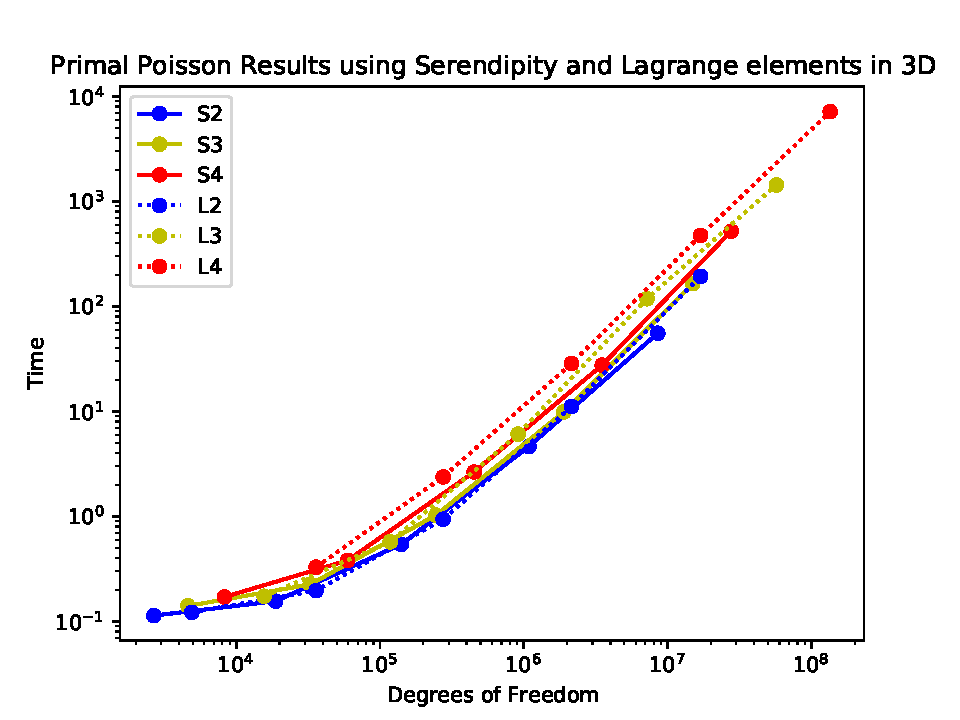
\includegraphics[height=2.2in]{3dPrimalDofsTime.pdf}
    \caption{3D Primal Degrees of freedom vs Time}
    \label{fig:3dPrimalDofsTime}
  \end{subfigure}
  ~
  \begin{subfigure}[h]{0.5\textwidth}
    \centering
    \begin{tikzpicture}[scale=0.88]
      \begin{loglogaxis}[xlabel={Time}, ylabel={Error},
             ylabel near ticks, ymax=1e-3, ymin=1e-11, xmax=1e4, xmin=0.5e-1,
             legend pos=north east, legend style={font=\tiny} ,
             cycle list name=color list, title={Primal Poisson using $S^-$ and $Q^-$}]
        %\addplot+[only marks, orange] table [x=Dofs,y=Time,col sep=comma]{PrimalPoissonSerendipity3dO4.csv};
        \addplot[red]
        table [x=Time,y=Error, col sep=comma]{PrimalPoissonSerendipity3dO2.csv};
        \addlegendentry{$S^-_2$}
        \addplot[blue] 
        table [x=Time,y=Error, col sep=comma]{PrimalPoissonSerendipity3dO3.csv};
        \addlegendentry{$S^-_3$ }
        \addplot[orange]
        table [x=Time,y=Error, col sep=comma]{PrimalPoissonSerendipity3dO4.csv};
        \addlegendentry{$S^-_4$}
        \addplot[densely dotted, red]
        table [x=Time,y=Error, col sep=comma]{PrimalPoissonLagrange3dO2.csv};
        \addlegendentry{$Q^-_2$}
        \addplot[densely dotted, blue] 
        table [x=Time,y=Error, col sep=comma]{PrimalPoissonLagrange3dO3.csv};
        \addlegendentry{$Q^-_3$}
        \addplot[densely dotted, orange]
        table [x=Time,y=Error, col sep=comma]{PrimalPoissonLagrange3dO4.csv};
        \addlegendentry{$Q^-_4$}
        
        \addplot+[only marks, red] table [x=Time,y=Error,col sep=comma]{PrimalPoissonSerendipity3dO2.csv};
        \addplot+[only marks, red, mark=square*] table [x=Time,y=Error,col sep=comma]{PrimalPoissonLagrange3dO2.csv};
        \addplot+[only marks, blue] table [x=Time,y=Error,col sep=comma]{PrimalPoissonSerendipity3dO3.csv};
        \addplot+[only marks, blue, mark=square*] table [x=Time,y=Error,col sep=comma]{PrimalPoissonLagrange3dO3.csv};
        \addplot+[only marks, orange] table [x=Time,y=Error,col sep=comma]{PrimalPoissonSerendipity3dO4.csv};
        \addplot+[only marks, orange, mark=square*] table [x=Time,y=Error,col sep=comma]{PrimalPoissonLagrange3dO4.csv};
      \end{loglogaxis}
      \end{tikzpicture}
    %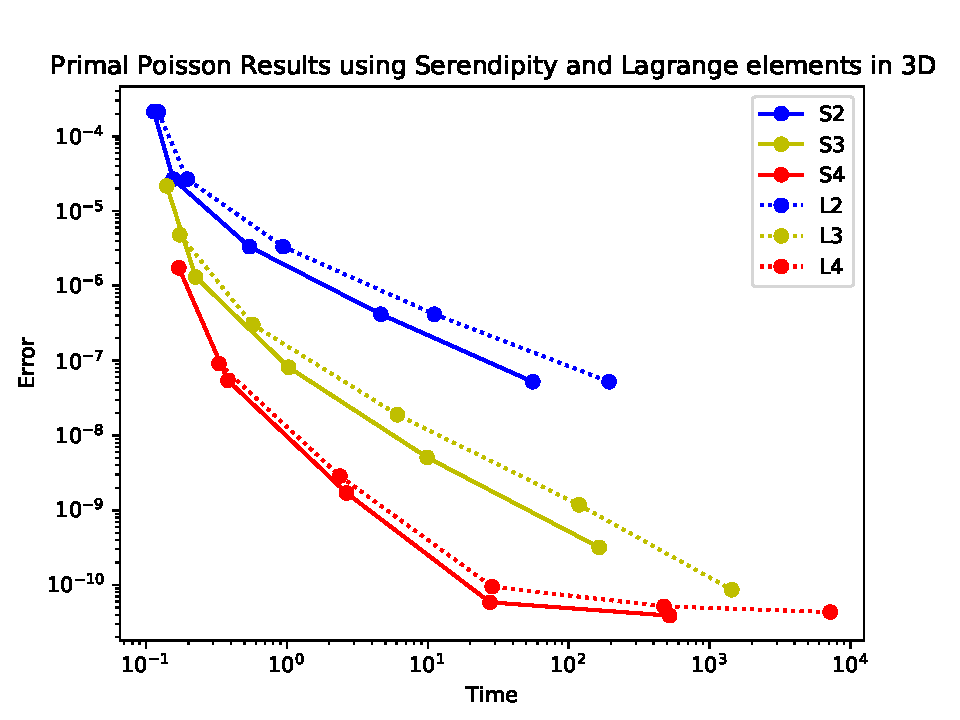
\includegraphics[height=2.2in]{3dPrimalTimeError.pdf}
    \caption{3D Primal Time vs Error}
    \label{fig:3dPrimalTimeError}
  \end{subfigure}\\
  ~
  \begin{subfigure}[h]{0.5\textwidth}
    \centering
    \begin{tikzpicture}[scale=0.88]
      \begin{loglogaxis}[xlabel={Degrees of Freedom}, ylabel={Time},
             ylabel near ticks, ymax=2e4, ymin=1e-1, xmax=2e7, xmin=0.5e4,
             legend pos=north west, legend style={font=\tiny} ,
             cycle list name=color list, title={Mixed Poisson using $S^-$ and $Q^-$}]
        %\addplot+[only marks, orange] table [x=Dofs,y=Time,col sep=comma]{PrimalPoissonSerendipity3dO4.csv};
        \addplot[red]
        table [x=Dofs,y=Time, col sep=comma]{MixedPoissonSminus3dO2.csv};
        \addlegendentry{$S^-_2$}
        \addplot[blue] 
        table [x=Dofs,y=Time, col sep=comma]{MixedPoissonSminus3dO3.csv};
        \addlegendentry{$S^-_3$ }
        \addplot[orange]
        table [x=Dofs,y=Time, col sep=comma]{MixedPoissonSminus3dO4.csv};
        \addlegendentry{$S^-_4$}
        \addplot[densely dotted, red]
        table [x=Dofs,y=Time, col sep=comma]{MixedPoissonNCF3dO2.csv};
        \addlegendentry{$Q^-_2$}
        \addplot[densely dotted, blue] 
        table [x=Dofs,y=Time, col sep=comma]{MixedPoissonNCF3dO3.csv};
        \addlegendentry{$Q^-_3$}
        \addplot[densely dotted, orange]
        table [x=Dofs,y=Time, col sep=comma]{MixedPoissonNCF3dO4.csv};
        \addlegendentry{$Q^-_4$}
        
        \addplot+[only marks, red] table [x=Dofs,y=Time,col sep=comma]{MixedPoissonSminus3dO2.csv};
        \addplot+[only marks, red, mark=square*] table [x=Dofs,y=Time,col sep=comma]{MixedPoissonNCF3dO2.csv};
        \addplot+[only marks, blue] table [x=Dofs,y=Time,col sep=comma]{MixedPoissonSminus3dO3.csv};
        \addplot+[only marks, blue, mark=square*] table [x=Dofs,y=Time,col sep=comma]{MixedPoissonNCF3dO3.csv};
        \addplot+[only marks, orange] table [x=Dofs,y=Time,col sep=comma]{MixedPoissonSminus3dO4.csv};
        \addplot+[only marks, orange, mark=square*] table [x=Dofs,y=Time,col sep=comma]{MixedPoissonNCF3dO4.csv};
      \end{loglogaxis}
      \end{tikzpicture}
    %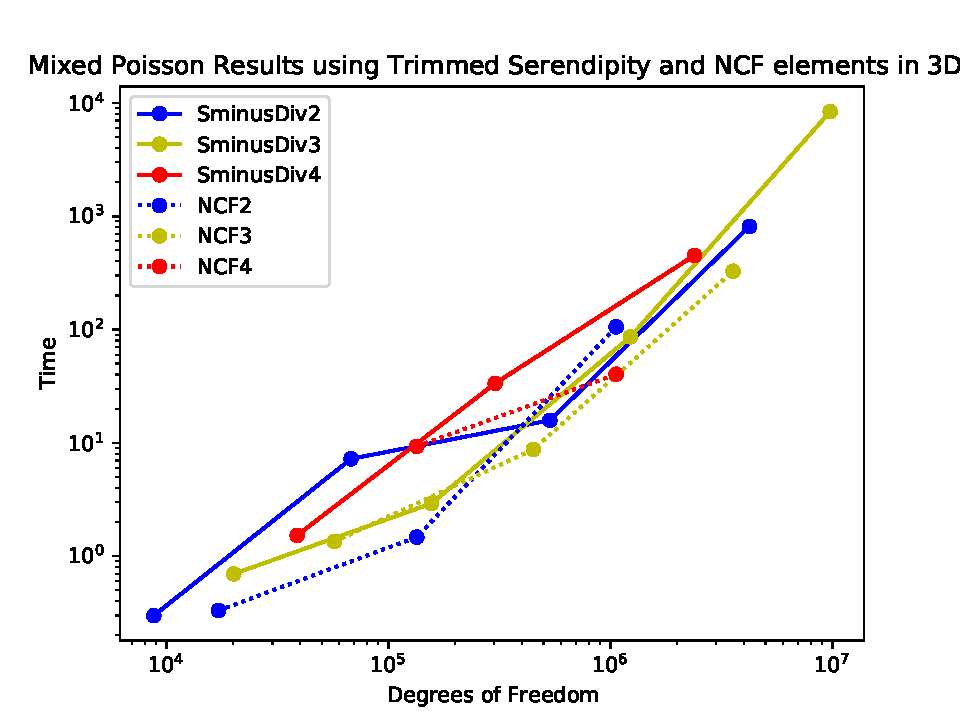
\includegraphics[height=2.2in]{3dMixedPoissonDofsTime.pdf}
    \caption{3D Mixed Degrees of freedom vs Time}
    \label{fig:3dMixedDofsTime}
  \end{subfigure}
  ~
  \begin{subfigure}[h]{0.5\textwidth}
    \centering
    \begin{tikzpicture}[scale=0.88]
      \begin{loglogaxis}[xlabel={Time}, ylabel={Error},
             ylabel near ticks, ymax=1e-1, ymin=5e-8, xmax=1e5, xmin=0.5e-1,
             legend pos=north east, legend style={font=\tiny} ,
             cycle list name=color list, title={Mixed Poisson using $S^-$ and $Q^-$}]
        %\addplot+[only marks, orange] table [x=Dofs,y=Time,col sep=comma]{PrimalPoissonSerendipity3dO4.csv};
        \addplot[red]
        table [x=Time,y=Error, col sep=comma]{MixedPoissonSminus3dO2.csv};
        \addlegendentry{$S^-_2$}
        \addplot[blue] 
        table [x=Time,y=Error, col sep=comma]{MixedPoissonSminus3dO3.csv};
        \addlegendentry{$S^-_3$ }
        \addplot[orange]
        table [x=Time,y=Error, col sep=comma]{MixedPoissonSminus3dO4.csv};
        \addlegendentry{$S^-_4$}
        \addplot[densely dotted, red]
        table [x=Time,y=Error, col sep=comma]{MixedPoissonNCF3dO2.csv};
        \addlegendentry{$Q^-_2$}
        \addplot[densely dotted, blue] 
        table [x=Time,y=Error, col sep=comma]{MixedPoissonNCF3dO3.csv};
        \addlegendentry{$Q^-_3$}
        \addplot[densely dotted, orange]
        table [x=Time,y=Error, col sep=comma]{MixedPoissonNCF3dO4.csv};
        \addlegendentry{$Q^-_4$}
        
        \addplot+[only marks, red] table [x=Time,y=Error,col sep=comma]{MixedPoissonSminus3dO2.csv};
        \addplot+[only marks, red, mark=square*] table [x=Time,y=Error,col sep=comma]{MixedPoissonNCF3dO2.csv};
        \addplot+[only marks, blue] table [x=Time,y=Error,col sep=comma]{MixedPoissonSminus3dO3.csv};
        \addplot+[only marks, blue, mark=square*] table [x=Time,y=Error,col sep=comma]{MixedPoissonNCF3dO3.csv};
        \addplot+[only marks, orange] table [x=Time,y=Error,col sep=comma]{MixedPoissonSminus3dO4.csv};
        \addplot+[only marks, orange, mark=square*] table [x=Time,y=Error,col sep=comma]{MixedPoissonNCF3dO4.csv};
      \end{loglogaxis}
      \end{tikzpicture}
    %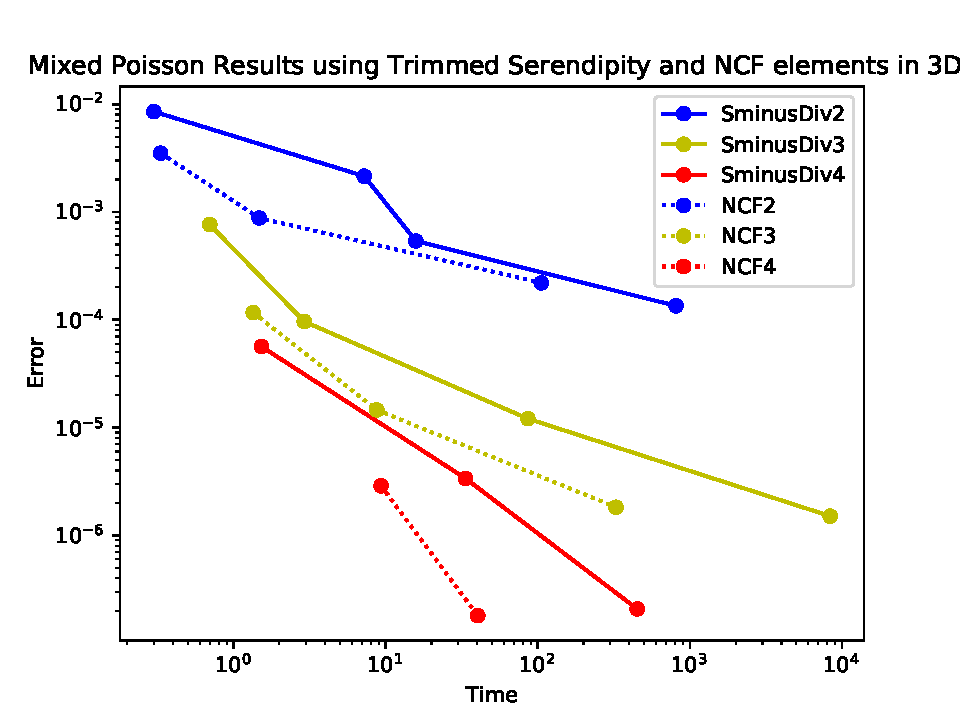
\includegraphics[height=2.2in]{3dMixedPoissonTimeError.pdf}
    \caption{3D Mixed Time vs Error}
    \label{fig:3dMixedTimeError}
  \end{subfigure}
  \caption{Analyzing timing data for primal and mixed Poisson problems using trimmed Serendipity and tensor product elements.}
\label{fig:PrimalMixedTimeAnalysis}
\end{figure}


\newpage  
  
\newpage 



\subsection{Cavity Resonator}

For testing the H$($curl$)$ elements in 3D, we use the cavity resonator problem.  Here, the time-harmonic Maxwell equations are applied to a domain $\Omega = [0,1]^3$ with perfectly conducting boundary conditions, yielding an eigenvalue problem where $\omega$ represents the resonances (i.e.\ eigenvalues) and $E$ represents the electric field (i.e.\ eigenfunctions):


\begin{equation}
    \langle \text{curl}(F), \text{curl}(E) \rangle = \omega^2 \langle F, E \rangle \text{ for all } F \in H_0(\text{curl}).
\end{equation}

%\noindent We tested out the H$($curl$)$ elements in 3D on the cavity resonator problem, where the time-harmonic Maxwell equations applied to a 
%\akg{(1) The wording is a little ambiguous - are you about the state the resonator problem or Maxwell's equations?  Or are these the same?  (2) I prefer to see the statement of the variables prior to the PDE i.e. move the part after the equation to before it. (3) You need to state the domain - I think it's $[0,1]^3\subset\R^3$ - and the boundary conditions (periodic?) (4) Give the eigenvalue equation a label so you can reference it later.}

The exact eigenvalues should follow the formula

\[ \omega^2 = m_1^2 + m_2^2 + m_3^2 \]

\noindent where $m_i \in \mathbb{N} \cup {0}$ and no more than one of $m_1, m_2, m_3$ may be equal to $0$ at a time \cite{rognes2010efficient}.

%\akg{Put discretized version of eigenvalue problem here (see comment below)}

\begin{center}
\begin{table}
\begin{tabular}{ c c c c c }
\multicolumn{5}{c}{NCE Elements} \\
\hline
Actual & N = 4 & N = 8 & N = 16 & N = 32 \\ 
\hline
2 &2.001024 & 2.000066 (3.96) & 2.000004 (4.04) & 2.0000003 (4.00) \\  
2 & 2.001024 & 2.000066 (3.96) & 2.000004 (4.04) & 2.0000003 (4.00)  \\
2 & 2.001024 & 2.000066 (3.96) & 2.000004 (4.04) & 2.0000003 (4.00)\\
3 & 3.001536 & 3.000098 (3.97) & 3.000006 (4.03) & 3.0000004 (4.02) \\
3 & 3.001536 & 3.000098 (3.97) & 3.000006 (4.03) & 3.0000004 (4.02) \\
5 & 5.030601 & 5.002081 (3.88)& 5.000133 (3.97) & 5.000008 (4.06) \\
5 & 5.030601 & 5.002081 (3.88)& 5.000133 (3.97) & 5.000008 (4.06) \\
5 & 5.030601 & 5.002081 (3.88) & 5.000133 (3.97) & 5.000008 (4.06) \\
5 & 5.030601 & 5.0002081 (3.88) & 5.000133 (3.97) & 5.000008 (4.06) \\
6 & 6.031114 & 6.002114 (3.88) & 6.000135 (3.97) &  6.000008 (4.08) \\
6 & 6.031114 & 6.002114 (3.88) & 6.000135 (3.97) & 6.000008 (4.08) \\
6 & 6.031114 & 6.002114 (3.88) & 6.000135 (3.97) & 6.000008 (4.08) \\
8 & - & -& - & - \\
\hline
Iterations & 4 & 4 & 3 & 5 \\
\hline
DOF  & 1944 & 13872 & 104544 & 811200 \\
\hline
EPS Solve Time (seconds) & 0.062609 & 0.297538 & 3.145271 & 38.093263 \\
\hline
\multicolumn{5}{c}{$S^-$ H$($curl$)$ Elements} \\
\hline
Actual & N = 4 & N = 8 & N = 16 & N = 32 \\ 
\hline
2 &2.001092 & 2.000066 (4.05) & 2.000004 (4.04) & 2.000000 (4.00) \\  
2 & 2.001092 & 2.000066 (4.05) & 2.000004 (4.04) & 2.000000 (4.00)  \\
2 & 2.001092 & 2.000066 (4.05) & 2.000004 (4.04) & 2.000000 (4.00)\\
3 & 3.009018 & 3.000586 (3.94) & 3.000037 (3.99) & 3.000002 (4.21) \\
3 & 3.009018 & 3.000586 (3.94) & 3.000037 (3.99) & 3.000002 (4.21) \\
5 & 5.032027 & 5.002097 (3.93)& 5.000133 (3.98) & 5.000008 (4.06) \\
5 & 5.032027 & 5.002097 (3.93)& 5.000133 (3.98) & 5.000008 (4.06) \\
5 & 5.032027 & 5.002097 (3.93) & 5.000133 (3.98) & 5.000008 (4.06) \\
5 & 5.032027 & 5.002097 (3.93) & 5.000133 (3.98) & - \\
6 & 6.072012 & 6.004976 (3.86) & 6.000319 (3.96) & 6.000020 (4.00) \\
6 & 6.072012 & 6.004976 (3.86) & 6.000319 (3.96) & 6.000024 (3.73)\\
6 & - & - & 6.00038 & 6.000024 (3.98)\\
8 & - & - & - & 8.000017 \\
\hline
Iterations & 4 & 5 & 4 & 3 \\
\hline
DOF  & 1080 & 7344 & 53856 & 411840 \\
\hline
EPS Solve Time (seconds) & 0.051549 & 0.154884 & 1.606652 & 12.599062 \\
\hline

\end{tabular}
\caption{A comparison of how order 2 NCE and $S^-$ finite elements solve the Maxwell cavity resonator eigenvalue problem, $\langle \text{curl}(F), \text{curl}(E) \rangle = \omega^2 \langle F, E \rangle$. }  
\label{tab:Eigenvalue}
\end{table}
\end{center}

In Table~\ref{tab:Eigenvalue}, we look at the convergence rates of different eigenvalues based off solving the problem with tensor product (NCE) elements and trimmed Serendipity ($S^-$) elements in 3D.  The table is split into two mirrored halves, the top half giving values from using NCE elements while the bottom half gives values from using $S^-$ elements.  The column labeled "Actual" represents the theoretical eigenvalue that eigenvalues in that row are converging towards.  Each of the $N=4, N=8, N=16, N=32$ columns represents the approximate eigenvalues calculated on a mesh of size $N x N x N$.  The number in parenthesis next to approximate eigenvalues is the rate of convergence of that eigenvalue.  Finally, each half has a row giving the overall degrees of freedom in the mesh at each given mesh size and another row that gives the time that the eigenvalue solver needed to find the requested number of eigenvalues.


Note that the convergence rates are computed by doing

\[r = \frac{\text{log}\bigg(\frac{\tilde{\lambda}_{i,N} - \lambda_{i,N}}{\tilde{\lambda}_{i,N+1} - \lambda_{i,N+1}} \bigg)}{\text{log}\bigg( \frac{h_N}{h_{N+1}} \bigg)} \]

\noindent and are indicated in the chart by using parentheses.  We use H$($curl$)$ to solve the problems, corresponding with edge elements in 3D.  Based off earlier eigenvalue works \cite{boffi2010finite}, we expect that the rate of convergence be double the order of the finite element used to solve the problem.  This is reflected in the table relatively well for both $S^-$ and NCE elements.\\

Any eigenvalue that has a $-$ spot is to be interpreted as the eigenvalue solver did not find that specific eigenvalue in the number of iterations it required to find the first 15 requested eigenvalue-eigenvector pairs.\\

The experiment was done by using SLEPc in Firedrake, computing an inverted shift to a target of $3.0$, then asking SLEPc for $15$ eigenvalue-eigenvector pairs.  SLEPc was then give a tolerance level of $1\text{e}-7$, and a couple of specific mumps parameters (icntl 14 set to 200 and icntl 13 set to 1).  We ignored the eigenvalues of $1$, as they correspond only to the boundary conditions. 

Knowing that both elements are solving this problem in a fashion that is expected theoretically, we can analyze the rest of the results shown in this table.  Investigating the error in the eigenvalues in the chart compared to the exact values, we see that NCE elements are able to get results that are up to a magnitude better near the target eigenvalue.  On the other hand, this loss of accuracy from using trimmed Serendipity elements results in a significant reduction in required time to solve for the requested eigenvalues.  At every mesh refinement level, trimmed Serendipity elements have nearly half the DOFs of NCE elements, and correspondingly, require about half the time to solve for the eigenvalues.  At higher orders, we expect that this will be even more exaggerated.  \\

\section{Conclusion}

Each finite element has a time and place where it could be considered beneficial to use.  We explored the numerical properties of trimmed Serendipity elements to refine our understanding of how they act.  From the theory, we knew that trimmed Serendipity elements should be able to converge at the same rate as tensor product and Serendipity elements, while using fewer degrees of freedom overall.  The plots here demonstrate that the rate of convergence is consistent with what we expect at many orders for H$($curl$)$, H$($div$)$, and $L^2$ elements in both 2 and 3D.\\

 Beyond the convergence rates hitting what we expect, we were able to analyze memory usage on these problems by studying the degrees of freedom required.  Trimmed Serendipity, while generally have a worse error at a given order $k$, also uses significantly fewer degrees of freedom.  This is illustrated well in the Maxwell Cavity Eigenvalue problem in \ref{tab:Eigenvalue}, where the degrees of freedom required were nearly half of what the tensor product elements used.  \\

 Another example of this is the 3D mixed Poisson problem, where we see that the trimmed Serendipity elements are able to be used at more refined meshes while the tensor product elements would need to be allotted more time on a high memory computer to be able to get results on the same sized mesh.  \\

In general, it is clear from these results that trimmed Serendipity is not always a better choice compared to tensor product elements.  However, these examples illustrates the benefit of trimmed Serendipity elements--in a setting where the mesh is fixed, the option to use a trimmed Serendipity element might give an extra way to refine a problem to increase the accuracy of a solution.



      \begin{tikzpicture}[scale=0.88]
      \begin{loglogaxis}[xlabel={Degrees of Freedom}, ylabel={Time},
             ylabel near ticks, ymax=1.e+4, ymin=0.5e-1, xmax=2.e8, xmin=1.e+3,
             legend pos=north west, legend style={font=\tiny} ,
             cycle list name=color list]
        %\addplot+[only marks, orange] table [x=Dofs,y=Time,col sep=comma]{PrimalPoissonSerendipity3dO4.csv};
        \addplot[red]
        table [x=Dofs,y=Time, col sep=comma]{PrimalPoissonSerendipity3dO2.csv};
        \addlegendentry{$S^-_2$}
        \addplot[blue] 
        table [x=Dofs,y=Time, col sep=comma]{PrimalPoissonSerendipity3dO3.csv};
        \addlegendentry{$S^-_3$ }
        \addplot[orange]
        table [x=Dofs,y=Time, col sep=comma]{PrimalPoissonSerendipity3dO4.csv};
        \addlegendentry{$S^-_4$}
        \addplot[densely dotted, red]
        table [x=Dofs,y=Time, col sep=comma]{PrimalPoissonLagrange3dO2.csv};
        \addlegendentry{$Q^-_2$}
        \addplot[densely dotted, blue] 
        table [x=Dofs,y=Time, col sep=comma]{PrimalPoissonLagrange3dO3.csv};
        \addlegendentry{$Q^-_3$}
        \addplot[densely dotted, orange]
        table [x=Dofs,y=Time, col sep=comma]{PrimalPoissonLagrange3dO4.csv};
        \addlegendentry{$Q^-_4$}
        
        \addplot+[only marks, red] table [x=Dofs,y=Time,col sep=comma]{PrimalPoissonSerendipity3dO2.csv};
        \addplot+[only marks, red, mark=square*] table [x=Dofs,y=Time,col sep=comma]{PrimalPoissonLagrange3dO2.csv};
        \addplot+[only marks, blue] table [x=Dofs,y=Time,col sep=comma]{PrimalPoissonSerendipity3dO3.csv};
        \addplot+[only marks, blue, mark=square*] table [x=Dofs,y=Time,col sep=comma]{PrimalPoissonLagrange3dO3.csv};
        \addplot+[only marks, orange] table [x=Dofs,y=Time,col sep=comma]{PrimalPoissonSerendipity3dO4.csv};
        \addplot+[only marks, orange, mark=square*] table [x=Dofs,y=Time,col sep=comma]{PrimalPoissonLagrange3dO4.csv};
      \end{loglogaxis}
      \end{tikzpicture}
      
      
      \begin{tikzpicture}[scale=0.88]
      \begin{loglogaxis}[xlabel={Degrees of Freedom}, ylabel={Error},
             ylabel near ticks, ymax=1e-1, ymin=2e-8, xmax=2e7, xmin=0.5e4,
             legend pos=south west, legend style={font=\tiny} ,
             cycle list name=color list, title={Mixed Poisson Error Analysis}]
        %\addplot+[only marks, orange] table [x=Dofs,y=Time,col sep=comma]{PrimalPoissonSerendipity3dO4.csv};
        \addplot[red]
        table [x=Dofs,y=Error, col sep=comma]{MixedPoissonSminus3dO2.csv};
        \addlegendentry{$S^-_2$}
        \addplot[blue] 
        table [x=Dofs,y=Error, col sep=comma]{MixedPoissonSminus3dO3.csv};
        \addlegendentry{$S^-_3$ }
        \addplot[orange]
        table [x=Dofs,y=Error, col sep=comma]{MixedPoissonSminus3dO4.csv};
        \addlegendentry{$S^-_4$}
        \addplot[densely dotted, red]
        table [x=Dofs,y=Error, col sep=comma]{MixedPoissonNCF3dO2.csv};
        \addlegendentry{$Q^-_2$}
        \addplot[densely dotted, blue] 
        table [x=Dofs,y=Error, col sep=comma]{MixedPoissonNCF3dO3.csv};
        \addlegendentry{$Q^-_3$}
        \addplot[densely dotted, orange]
        table [x=Dofs,y=Error, col sep=comma]{MixedPoissonNCF3dO4.csv};
        \addlegendentry{$Q^-_4$}
        
        \addplot+[only marks, red] table [x=Dofs,y=Error,col sep=comma]{MixedPoissonSminus3dO2.csv};
        \addplot+[only marks, red, mark=square*] table [x=Dofs,y=Error,col sep=comma]{MixedPoissonNCF3dO2.csv};
        \addplot+[only marks, blue] table [x=Dofs,y=Error,col sep=comma]{MixedPoissonSminus3dO3.csv};
        \addplot+[only marks, blue, mark=square*] table [x=Dofs,y=Error,col sep=comma]{MixedPoissonNCF3dO3.csv};
        \addplot+[only marks, orange] table [x=Dofs,y=Error,col sep=comma]{MixedPoissonSminus3dO4.csv};
        \addplot+[only marks, orange, mark=square*] table [x=Dofs,y=Error,col sep=comma]{MixedPoissonNCF3dO4.csv};
      \end{loglogaxis}
      \end{tikzpicture}


\bibliographystyle{ACM-Reference-Format}  %Might need acmart.cls (unclear)
\bibliography{serendipityFiredrakePaper}  %Change this to the bib file

\end{document}